\documentclass[tikz,border=5pt]{standalone}
\usepackage{tikz}
\usetikzlibrary{arrows.meta,positioning,calc}
\definecolor{nebula}{HTML}{6366F1}
\definecolor{spark}{HTML}{14B8A6}
\definecolor{ink}{HTML}{334155}
\begin{document}
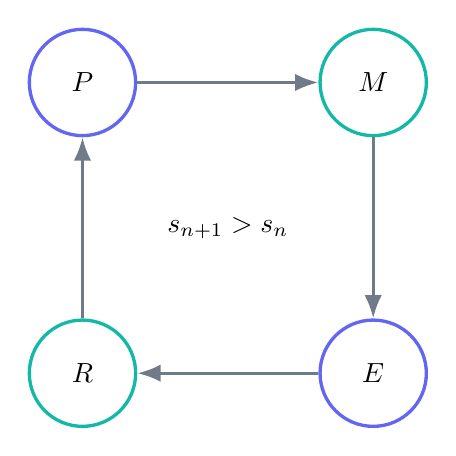
\begin{tikzpicture}[font=\sffamily,>=Latex,node distance=2.3cm]
  \node[draw=nebula,very thick,circle,minimum size=1.35cm] (p) {$P$};
  \node[draw=spark,very thick,circle,minimum size=1.35cm,right=of p] (m) {$M$};
  \node[draw=nebula,very thick,circle,minimum size=1.35cm,below=of m] (e) {$E$};
  \node[draw=spark,very thick,circle,minimum size=1.35cm,left=of e] (r) {$R$};
  \draw[->,very thick,ink!70] (p)--(m);
  \draw[->,very thick,ink!70] (m)--(e);
  \draw[->,very thick,ink!70] (e)--(r);
  \draw[->,very thick,ink!70] (r)--(p);
  \node[fill=white,inner sep=4pt] at ($(p)!0.5!(e)$) {$s_{n+1}>s_n$};
\end{tikzpicture}
\end{document}
